\documentclass[nofootinbib,amssymb,amsmath]{revtex4}
\usepackage{mathtools}
\usepackage{amsthm}
\usepackage{algorithm}
\usepackage{algpseudocode}
\usepackage{lmodern}
\usepackage{graphicx}
\usepackage{color}

%Put an averaged random variable between brackets
\newcommand{\ave}[1]{\left\langle #1 \right\rangle}

\newtheorem{lemma}{Lemma}
\newtheorem{corollary}{Corollary}

\def\SL#1{{\color [rgb]{0,0,0.8} [SL: #1]}}
\def\DB#1{{\color [rgb]{0,0.8,0} [DB: #1]}}

\begin{document}

\title{Notes on CNV Methods}
\author{David Benjamin}
\email{davidben@broadinstitute.org}
\affiliation{Broad Institute, 75 Ames Street, Cambridge, MA 02142}

\author{Samuel K. Lee}
\email{slee@broadinstitute.org}
\affiliation{Broad Institute, 75 Ames Street, Cambridge, MA 02142}

\date{\today}

\begin{abstract}
Some notes on current and proposed methods used in the GATK CNV and ACNV workflows.
\end{abstract}

\maketitle

\section{Introduction}\label{introduction}

The GATK uses two types of information from sequencing data to detect copy number variations (CNVs).  First, targets (usually exons but in principle any genomic locus) with abnormally high or low coverage suggest amplifications or deletions, respectively.  Second, sites that are heterozygous in a normal sample and have allele ration significantly different from 1:1 in the matched tumor sample imply a CNV event involving one or both alleles.  The workflow is as follows:

\begin{enumerate}

\item Partition targets into continuous segments that represent the same copy-number event using coverage data.  The segmentation is performed by a circular-binary-segmentation (CBS) algorithm described by Olshen et al. 2004 that was originally developed to segment noisy array copy-number data.\footnote{Specifically, the CBS implementation provided by the \texttt{R} package \texttt{DNACopy} is used.}

\item Find heterozygous sites in the normal case sample and segment these, again using CBS, according to their ref:alt allele ratios in the tumor sample.

\item Combine the two sets of segments in a liberal manner that tends to produce too many segments.

\item Alternate between modeling the copy ratio and minor allele fraction of each segment with merging adjacent segments that are sufficiently similar according to this model.

\end{enumerate}

\section{Segmentation by Coverage and Minor Allele Fraction} \label{recapseg-overview}

\subsection{Panel of Normals}
We cannot simply divide the coverage of each target by the average sequencing depth to obtain an estimate of its copy ratio.  The coverage of different targets is heavily-biased by factors including the efficiency of their baits, GC content, and mappability.  In order to detect CNVs we must model the coverage of each target in the absence of CNVs, which requires a panel of normal samples (PoN) that are representative of the sequencing conditions of the case sample.  PoN samples must be created using the same baits as the case sample.  The steps for creating a panel of normals are

\begin{enumerate}

\item  Obtain the coverage (total number of overlapping reads) of every target and sample.

\item Calculate the median coverage of each target over all samples.

\item  Filter out targets whose median coverage is below a given percentile (by default 25\%) of target medians.

\item  Divide all coverages by their corresponding target medians.

\item Filter out samples with too great a proportion of zero-coverage targets (by default 5\%).

\item Filter out targets with zero coverage in too great a proportion of samples (by default 2\%).

\item Filter out samples whose median coverage is above or below certain percentiles (by default 2.5\% and 97.5\%) of sample medians.

\item Replace all remaining zero coverages with their corresponding target median. 

\item Calculate the range of coverage from percentile $p$\% to $(100 - p)$\% for each target and truncate coverages at each target to lie within these ranges.  By default $p = 0.1$.

\item Divide each coverage by its sample median.

\item Take the $\log_2$ of each coverage.

\item Calculate the median of each sample and take the median of these over all targets.  Subtract this median of medians from each coverage.

\item Perform a singular value decomposition (SVD) of the resulting matrix and calculate its pseudo-inverse truncated to the space spanned by the $k$ right eigenvectors with largest singular values. Choose $k$ using Jollife's heuristic of retaining singular values greater than 0.7 times the mean singular value.

\end{enumerate}

The output is: a $N \times k$ matrix $P$, the columns of which are the the retained right eigenvectors (eigensamples), and its pseudoinverse $P^+$; and the target medians (before any transformations).  Here $N$ denotes the number of targets.

\subsection{Segmentation by tangent-normalized coverage}
We first divide the integer coverage of the case sample at each target by the corresponding target median from the PoN and take the $\log_2$ transformation to obtain an $N \times 1$ column matrix ${\bf x}$.  We then calculate the ``tangent-normalized'' coverage: ${\bf x} - PP^+ {\bf x}$.  The meaning of this is as follows: $PP^+$ is an operator that projects onto the column space of $P$.  That is, it projects onto the space spanned by the $k$ most significant eigensamples representing the (non-CNV-related) variability of the coverage.  Subtracting the projection $PP^+ {\bf x}$ therefore isolates the CNV signal and removes noise due to fluctuations in sequencing bias.

Finally, the tangent-normalized coverage vector is passed to CBS to obtain coverage segments.

\subsection{Het coverage and segmentation by minor allele fraction}
Given a large database of common SNPs, we search the normal control sample for heterozygous sites.  To determine whether a site with $r$ ref reads and $a$ alt reads is heterozygous, we calculate the two-sided $p$-value under the null hypothesis that the number of alt reads follows a binomial distribution: $a \sim {\rm Binom}(a + r, 1/2)$.  If the $p$-value is not too small we consider the site heterozygous.

Ref and alt counts are then obtained at these sites in the tumor case sample.  To obtain initial minor-allele-fraction segments, we estimate the minor allele fraction for each het site by taking the maximum-likelihood estimate given by Equation~\ref{likelihood} with allelic bias ignored (i.e., $\lambda_j = 1$) and pass the resulting list to CBS.

\subsection{Target/SNP segment union} \label{targetsnp-segment-union}

\SL{SL will fill this in.}

\subsection{Small-segment merging} \label{small-segment-merging}

\SL{SL to update this to the new method.}

Using CBS to segment the targets in GATK CNV results in segments that are larger than a specified minimum number of targets $n_t$ (by default, $n_t = 2$).  However, after taking the union of target and SNP segments, small segments with less than $n_t$ targets may be introduced.  To be consistent with CBS and CNV, ACNV treats these small segments as spurious, and removes them by merging them with adjacent segments.

\section{GATK CNV/ACNV Models} \label{models}

\subsection{Copy-ratio model} \label{copy-ratio-model}

\SL{SL will fill this in.}

\subsection{Allelic model} \label{allelic-model}
We want a generative model for allelic fractions that infers its parameters from the data.  We observe alt and ref read counts for each het site and wish to infer the minor allelic fraction of every segment.  Let's consider what other hidden variables belong in the model.  Read counts obey an overdispersed binomial distribution in which the probability of an alt read is a site-dependent random variable.  Letting $\theta_j$ be the probability that a mapped read at het $j$ is an alt we have
%
\begin{equation}
P(a_j, r_j | \theta_j) =  \binom{a_j + r_j}{a_j} \theta_j^{a_j} (1-\theta_j)^{r_j} = \binom{n_j}{a_j} \theta_j^{a_j} (1-\theta_j)^{r_j},
\end{equation}
where $a_j$ and $r_j$ are alt and ref read counts and $n_j = a_j + r_j$ is the total read count at site $j$.  Now we consider $\theta_j$.  Suppose site $j$ belongs to a segment with minor allelic fraction $f$ and is alt minor, such that $P({\rm alt}) = f$ and $P({\rm ref}) = 1 - f$ are the probabilities that a random DNA fragment will contain the alt and ref alleles.  Let $x^{\rm alt (ref)}_j = P({\rm mapped} | {\rm alt (ref)})$ be the probabilities that an alt (ref) DNA fragment at site $j$ eventually gets sequenced and mapped.  Then $\theta_j$ is the conditional probability that a mapped read comes from an alt fragment:
%
\begin{align}
\theta_j  &= P( {\rm alt} | {\rm mapped} ) = \frac { P( {\rm alt} ) P( {\rm mapped} | {\rm alt} ) } { P( {\rm alt} ) P( {\rm mapped} | {\rm alt} ) + P( {\rm ref} ) P( {\rm mapped} | {\rm ref} ) } \\
 &= \frac{f x^{\rm alt}_j }{fx^{\rm alt} + (1-f) x^{\rm ref}_j } = \frac{f}{f + (1-f) \lambda_j},
\end{align}
%
where $\lambda_j = x^{\rm ref}_j / x^{\rm alt}_j$ is the ``bias ratio'' of ref to alt sequenceability and mappability at site $j$.  A similar result for ref minor sites follows from substituting $f \leftrightarrow 1 - f$.  In addition to the bias ratio $\lambda_j$ we need an indicator variables $z_j$ with three states, alt minor, ref minor, and an outlier state that gives robustness to anomalous events.  For this outlier state we average the binomial likelihood over all $\theta$ to get:
%
\begin{align}
P(a_j, r_j | {\rm outlier}) = \binom{n_j}{a_j} \int_0^1 \theta_j^{a_j} (1-\theta_j)^{r_j} \, d \theta_j 
= \binom{n_j}{a_j} \frac{a_j! r_j!}{(n_j + 1)!}
\end{align}
%
For notational convenience we give $z_j$ a one-of-$K$ encoding $z_j = (z_{ja}, z_{jr}, z_{jo})$ in which one component equals $1$ and the rest $0$.

The contribution of site $j$ to the likelihood is
%
\begin{equation}
P(a_j, r_j | f_j, \lambda_j, z_j) =  \binom{n_j}{a_j}  
\left[ \frac{f_j^{a_j} (1 - f_j)^{r_j} \lambda_j^{r_j}}{ \left( f_j + (1-f_j) \lambda_j \right)^{n_j}} \right]^{z_{ja}}   
\left[ \frac{(1-f_j)^{a_j} f_j^{r_j} \lambda_j^{r_j}}{ \left( 1 - f_j + f_j \lambda_j \right)^{n_j}} \right]^{z_{jr}}   
\left[ \frac{a_j! r_j!}{(n_j + 1)!} \right]^{z_{jo}}
\label{likelihood}
\end{equation}
%
where $f_s$ is the minor allele fraction of the segment containing site $j$.  We will consider $f$ to be drawn from a uniform distribution on $[0, 1/2]$ -- that is, we give it a flat prior -- but in the future we can obtain some sort of clustering behavior, representing the fact that events in the same subclone that exhibit the same integer copy numbers will have the same minor allelic fractions, by drawing $f_s$ from a Dirichlet process.

We assume that the bias ratios come from a common Gamma distribution with parameters $\alpha, \beta$:
%
\begin{equation}
P(\lambda_j | \alpha, \beta) = \frac{\beta^\alpha}{\Gamma(\alpha)} \lambda_j^{\alpha-1} e^{-\beta \lambda_j}
\end{equation}
%
Note that bias ratios tend to be near $1.0$ and so the choice of distribution is not too important as long as it has adjustable mean and standard deviation.  We choose the Gamma distribution because it is the simplest such distribution on $\mathbb{R}^+$.  We will give the parameters $\alpha$ and $\beta$ a flat prior $P(\alpha, \beta) \propto 1$.

Finally, the indicator $z_j$ is a multinomial random variable distributed according to parameter vector ${\bf \pi}$:
%
\begin{equation}
P(z_{ja(r,o)} = 1 | {\bf \pi}) = \pi_{a(r,o)}
\end{equation}
We set the alt and ref minor probabilities equal so that the only free parameter is $\pi = \pi_o$, with $\pi_{a(r)} = (1 - \pi)/2$.
%
The Bayesian network corresponding to this model is shown in Figure \ref{graphical_model}.
\begin{figure}
$
\begin{array}{c}
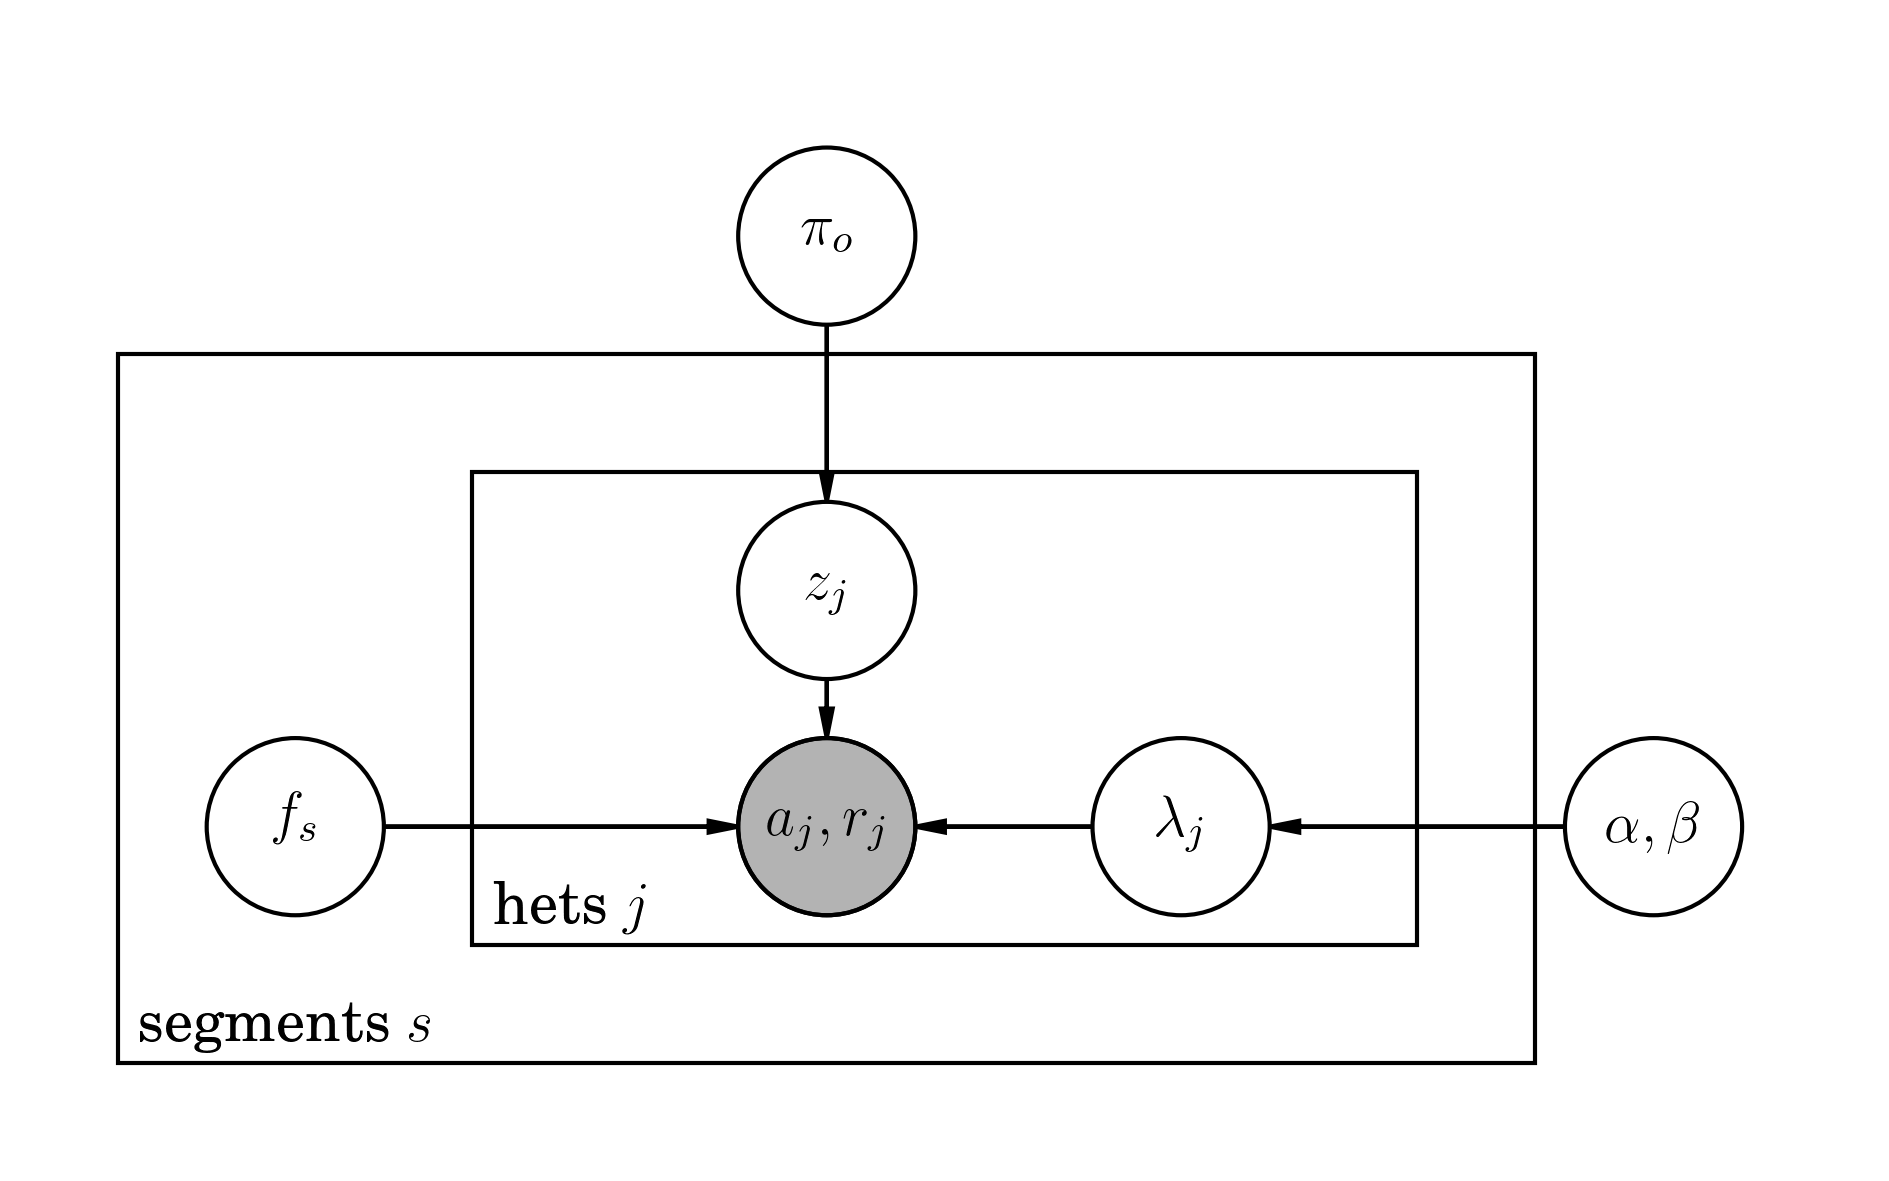
\includegraphics[width=0.8\linewidth]{ACNV_model.png} 
\end{array}
$
\label{graphical_model}
\caption{Graphical model for ACNV allelic model} 
\end{figure}

As with the other parameters, we put a flat prior on ${\rm \pi}$.  Putting all the pieces together the likelihood is
\begin{equation}
\mathbb{L} =\prod_j \frac{\beta^\alpha}{\Gamma(\alpha)} \lambda_j^{\alpha - 1} e^{-\beta \lambda_j}
\left[ \frac{(1-\pi) f_j^{a_j} (1 - f_j)^{r_j} \lambda_j^{r_j}}{ \left( f_j + (1-f_j) \lambda_j \right)^{n_j}} \right]^{z_{ja}}   
\left[ \frac{(1-\pi) (1-f_j)^{a_j} f_j^{r_j} \lambda_j^{r_j}}{ \left( 1 - f_j + f_j \lambda_j \right)^{n_j}} \right]^{z_{jr}}   
\left[ \frac{2 \pi a_j! r_j!}{(n_j + 1)!} \right]^{z_{jo}}.
\label{likelihood}
\end{equation}
%
The dependence on $\lambda$ for alt minor sites is
%
\begin{equation}
g(\lambda_j, \alpha, \beta, f_j, a_j, r_j) = \frac{\beta^\alpha}{\Gamma(\alpha)}  \frac{ f_j^{a_j} (1 - f_j)^{r_j}  \lambda_j^{\alpha + r_j - 1} e^{-\beta \lambda_j}}{ \left( f_j + (1-f_j) \lambda_j \right)^{n_j}}.
\end{equation}
For ref minor sites the dependence is the same but with $f \leftrightarrow 1 - f$.  We show in show in Appendix \ref{marginalizing} that this function can be integrated analytically, and thus we can marginalize $\lambda$ out of the model to obtain the likelihood
%
\begin{equation}
\prod_j 
\left[ \frac{1-\pi}{2} \phi(\alpha, \beta, f_j, a_j, r_j)  \right]^{z_{ja}}   
\left[ \frac{1-\pi}{2} \phi(\alpha, \beta, 1 - f_j, a_j, r_j)  \right]^{z_{jr}}   
\left[ \frac{ \pi a_j! r_j!}{(n_j + 1)!}  \right]^{z_{jo}},
\label{marginalized}
\end{equation}
%
where $\phi(\alpha, \beta, f_j, a_j, r_j) = \int_0^\infty g(\lambda, \alpha, \beta, f, a, r) \, d \lambda_j$.  Pseudocode for computing $\phi$ is presented in Appendix \ref{marginalizing}.  Furthermore, marginalizing out $z$ is trivial -- simply sum each term over its three possible states.  We then have a collapsed likelihood
%
\begin{equation}
p(f,\alpha, \beta, \pi) \propto \prod_j 
\left[    \frac{1-\pi}{2} \phi(\alpha, \beta, f_j, a_j, r_j)  +
\frac{1-\pi}{2} \phi(\alpha, \beta, 1 - f_j, a_j, r_j)  +
 \frac{ \pi a_j! r_j!}{(n_j + 1)!}    \right]
 \label{collapsed}
\end{equation}
%
Integrating out the latent variables removes the strongest correlations from the model -- intuitively, $f$ should not be too sensitive to $\alpha$ and $\beta$, for example -- and significantly improves mixing.  The exception is $\alpha$ and $\beta$, since adjusting one with the other fixed changes the mean of the prior on $\lambda$.  Thus we reparameterize in terms of $\mu$ and $\sigma^2$, the mean and variance of the common gamma distribution of biases, where $\alpha = \mu^2 / \sigma^2$ and $\beta = \mu / \sigma^2$.  Due to the weak correlations our MCMC method does not need to be very sophisticated.  We choose to sample each variable with one-dimensional adaptive Metropolis, tuning the proposal step size to achieve some reasonable acceptance rate like $0.4$ or so.  Thus we have completely specified an MCMC scheme for this model, given by Algorithm \ref{ACNV_MCMC}:

\begin{algorithm}
\begin{algorithmic}[1]
\State Initialize all parameters to a maximum likelihood initial guess (see below).
\Repeat
	\State Sample each $f_s$ with adaptive Metropolis
	\State Sample $\pi$ with adaptive Metropolis
	\State Sample $\mu$ with adaptive Metropolis
	\State Sample $\beta$ with adaptive Metropolis
\Until{convergence}
\end{algorithmic}
\caption{MCMC algorithm for ACNV allelic model}
\label{ACNV_MCMC}
\end{algorithm}

We initialize the model by finding the mode of likelihood.  This significantly reduces burn-in time of our MCMC sampling.  Also, it allows us to give the adaptive Metropolis samplers better initial guesses for their step sizes.  Since in practice there is a single global maximum of the likelihood it is easy to find.  After initializing the initialization with rough guesses for the parameters, we successively find one-dimensional maxima adjusting one parameter at a time until the likelihood converges.  One could use multidimensional optimization to obtain faster convergence, but after marginalizing out latent parameters the remaining correlations are weak and thus this simple approach performs quite well.  Since we may delegate one-dimensional maximization to mathematical libraries, the only thing left to describe is our initial coarse guess.

In the initial guess we set the outlier probability $\pi_o = 0.01$, $\mu = 1.0$, and $\sigma^2 = 0.1$.  With the exception of $\sigma^2$ these are all reasonable guesses.  We choose $\sigma^2$ to be larger than what we actually believe because $\mu$ converges more slowly from a bad initial guess if $\sigma^2$ is too small.  The only non-trivial part of the initial guess is the minor allele fractions.  For each segment, we wish to set the minor allele fraction to the number of reads from minor alleles divided by to total number of reads -- this is an unbiased estimator if allelic bias is absent.  The problem is that we have counts of alt and ref reads, not minor and major reads.  Our solution is to weight the alt and ref read counts on each het by probabilities that the het is alt and ref minor, respectively.  That is, we set
%
\begin{equation}
f_S \approx \frac{ \sum_{j \in S} a_j P(z_{ja} = 1) + r_j  P(z_{jr} = 1) }{ \sum_{j \in S} (a_j + r_j) (P(z_{ja} = 1) +  P(z_{jr}=1))}
\end{equation}
%
For this coarse guess we ignore the possibility of outliers, so that $P(z_{ja} = 1) +  P(z_{jr}=1) = 1$.  Ignoring bias and outliers the alt minor likelihood of het $j$ is proportional to $f_j^{a_j} (1-f_j)^{r_j}$.  Since we don't know $f$ yet, we integrate this (including the normalization) from $f=0$ to $f=1/2$ in order to get $P(z_{ja} = 1)$.  This quantity is called the incomplete regularized beta function $I$.  Thus we have
%
\begin{equation}
P(z_{ja} = 1) \approx I(1/2, a_j + 1, r_j + 1), \quad P(z_{jr} = 1) = 1 - P(z_{ja} = 1).
\end{equation}


\subsection{Calling segments after allelic CNV workflow} \label{ACNV-caller}
After running the allelic fraction and copy ratio model, we have a list of segments $s$, each with its own posterior pdfs $f_s^{\rm CR}$ and $f_s^{\rm MAF}$ of the copy ratio and minor allele fraction\footnote{ACNV obtains MCMC samples from these posteriors; we assume that a reasonable distribution has been fit to these posterior samples.}.  That is, $f_s^{MAF}(x)$ is the posterior probability density from ACNV that segment $s$ has minor allele fraction $x$.  We assume that for each segment some fraction $\rho$ of sequenced cells carry $m$ and $n$ copies of the original homologs, while the remaining $1 - \rho$ cells are diploid.  This assumption is compatible with both normal contamination and tumor heterogeneity but not with distinct subclones containing different CNVs at overlapping segments.  It \textit{can} express distinct subclones that inherit a CNV from a common ancestor, as well as a single subclone that incurs overlapping CNVs as long as both are fixed (in the population genetics sense) in that subclone.

Each distinct value of $\rho$ therefore corresponds to a node in the tumor's phylogenetic tree, its value being the proportion of sequenced cells belonging to subclones descended from that node.  We therefore expect its values to be drawn from a discrete multinomial distribution, on which we place a symmetric and sparse Dirichlet prior.  That is, let $\rho$ take on values $\rho_1, \rho_2 \ldots \rho_K$ and let $z_s$ be a binary-valued indicator vector such that $z_{sk} = 1$ if the CNV on segment $s$ occurs in fraction $\rho_k$ of sequenced cells.  Then
\begin{align} 
P(\pi | \alpha) =& \frac{ \Gamma(\alpha) }{\Gamma(\alpha/K)^K} \prod_k \pi_k^{\alpha/K - 1} \\
P(z_s | \pi) =& \prod_k \pi_k^{z_{sk}}
\end{align}
Here $\alpha$ is the concentration parameter such that the smallness of $\alpha / K$ enforces sparseness\footnote{If $\alpha < K$ the prior is singular as $\pi_k \rightarrow 0$ for any $k$.}, i.e. most cluster components will not be used.  The $K \rightarrow \infty$ limit is a Dirichlet process and for finite $K$ to work well, $K$ must be larger than the number of components needed; in practice making $K$ twice as large as the number of components works well.  The expected number of clusters found in data of size $N$ (here, the number of segments) is roughly $\alpha \ln N$, so we place a vague prior on $\alpha$ that corresponds to roughly a single- or double-digit number of clusters.  For example, a broad gamma prior with mean $1$:
%
\begin{equation}
P(\alpha) = {\rm Gamma}(\alpha | 1,1)
\end{equation}
%
We have little prior knowledge on tumor's phylogeny, so we put a uniform prior on the values of $\rho$: $P(\rho_k) = 1$.

Next we relate copy ratio and minor allele fraction to $(m, n, \rho)$.  The total copy number is a weighted sum of $(1-\rho)$ diploid cells and $\rho$ cells with copy number $m+n$.  
%
\begin{equation}
{\rm cr}(m, p, \rho) \equiv \left( 2(1-\rho) + \rho(m + n) \right)/2.
\end{equation}
%
Similarly, the minor allele fraction is a weighted sum of $1 - \rho$ diploid cells with a single copy of the minor allele and $\rho$ cells with ${\rm min}(m,n)$ copies, divided by the total:
%
\begin{equation}
{\rm maf}(m, n, \rho) \equiv \frac{(1- \rho) + \rho ~ {\rm min}(m,n)}{2(1-\rho) + \rho (m + n)}
\end{equation}
%
It is convenient to represent the latent state $(m,n)$ via binary indicator variables $v$ and $w$ with e.g. $v_{sm} = 1, w_{sn} = 1$ if segment $s$ has $m$ and $n$ copies of the original homologs.

Finally, we place a simple factorized multinomial prior on $(m,n)$: $P(m,n) = P(m)P(n) = \phi_m \phi_n$, which we can do if we set of maximum copy number of, say, $m, n < 4$.  The factorization assumption realistic regarding the origin of CNVs but not necessarily regarding their \textit{viability}.  For example, a homozygous deletion could be lethal when a heterozygous deletion is not.  However, we expect this effect to be less dramatic for small segments, which have less phenotypic impact.  Large segments ought to have sufficient statistical power that the prior is less important.  Taking into account the copy ratio and minor allele fraction posteriors from ACNV as well as the mulitnomial prior, the model likelihood is
%
\begin{equation}
P(z_s, v_s, w_s, \pi, \phi, \rho, \alpha) = P(\alpha) \frac{ \Gamma(\alpha) }{\Gamma(\alpha/K)^K} \prod_k \pi_k^{\alpha/K - 1} \prod_{s, k,n,m} \left[ \pi_k \phi_m \phi_n f_s^{\rm CR}({\rm cr}(m,n,\rho_k) f_s^{\rm MAF}({\rm maf}(m,n,\rho_k) \right]^{z_{sk} v_{sm} w_{sn}}
\end{equation}
%

Note that we have simply multiplied of contributions of copy number and minor allele fraction.  This is justified because we inferred the former only from total read counts, while the inference for the latter was \textit{conditioned} on the total read depth of each het.  Thus there is no double-counting of evidence.  This argument is somewhat heuristic because ACNV infers copy number from \textit{target} read counts and minor allele fraction from \textit{SNP} allele counts, but is valid to the extent that total depth at het sites is correlated with depth and the targets they belong to.  For off-target SNPs it is not heuristic at all.

The graphical model is shown in Figure \ref{acnv_caller_fig}.

\begin{figure}
$
\begin{array}{c}
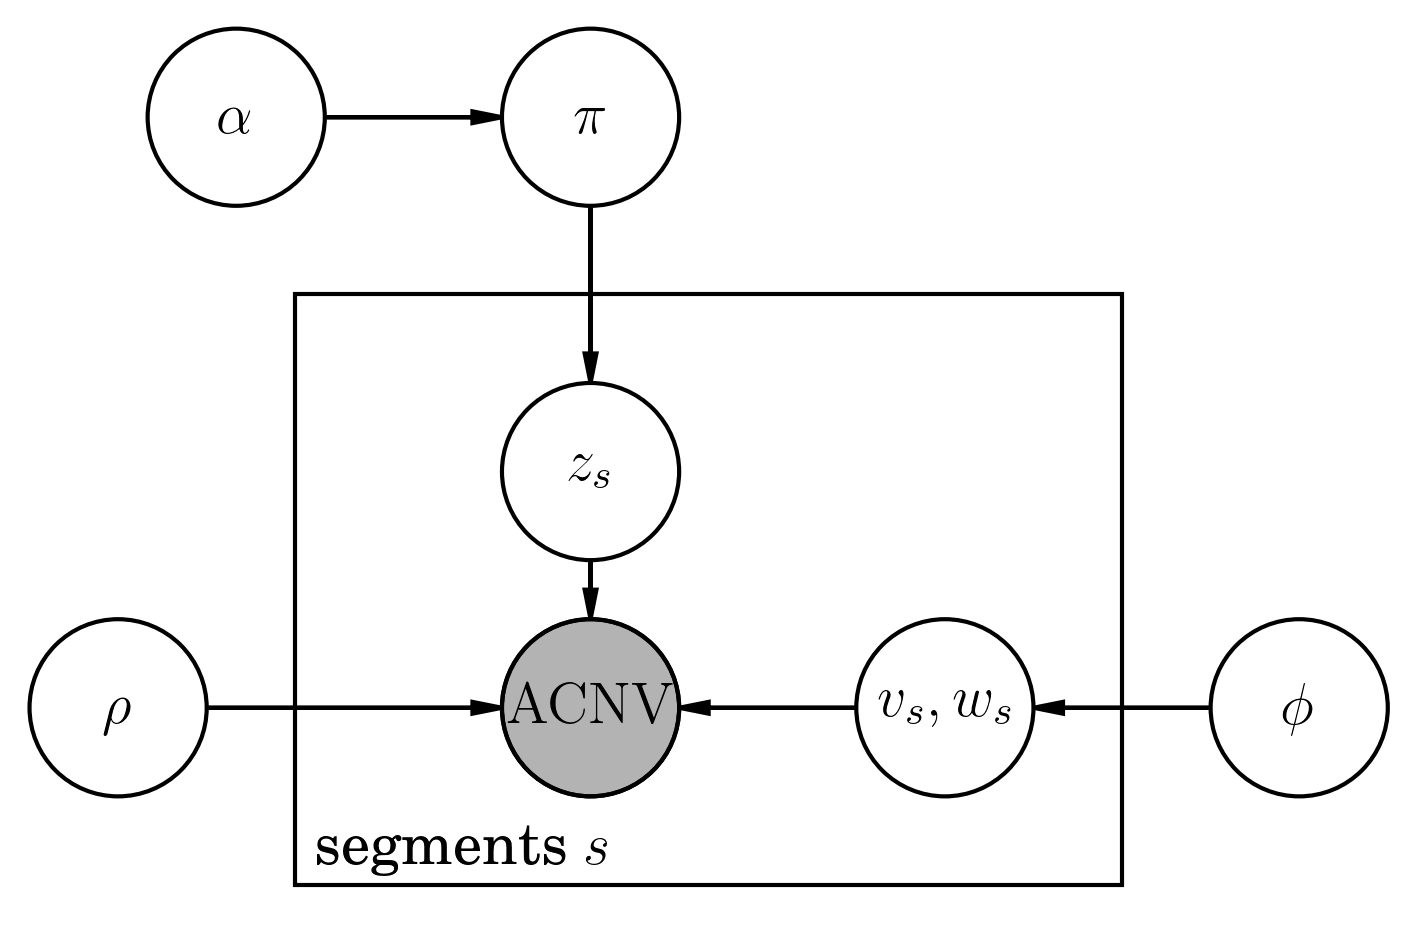
\includegraphics[width=0.8\linewidth]{ACNV_caller_model.png} 
\end{array}
$
\label{acnv_caller_fig}
\caption{Graphical model for ACNV caller.  ``ACNV" represents posterior probability output of ACNV; $v,w$ are indicators of homolog integer copy numbers; $\rho$ is the set of values of ${\rm purity} \times {\rm cancer~cell~fraction}$; $z$ is the corresponding indicator; $\phi$ is the multinomial prior on homolog counts; $\pi$ is the multinomial prior on $z$; $\alpha$ is a Dirichlet concentration parameter encouraging a sparse set of $\rho$ values.} 
\end{figure}

We will obtain maximum likelihood estimates of $\rho$ and $\phi$ and give the remaining variables the variational factorized distribution $p(\alpha, \pi, z, v, w) \rightarrow q(\alpha) q(\pi) q(z,v,w)$. We now proceed to carry out the standard recipe of the EM and variational Bayes algorithms.  Denoting one variable or group of variables by $X$, all other variables by $Z$, and the joint probability by $p(X,Z)$, the mean-field posterior on $X$ is
%
\begin{equation}
\ln q(X) = E_{q(Z)}[\ln p(X,Z)] + {\rm const}
\end{equation}
%
For those variables $X$ for which we seek a point estimate and not a full posterior we employ a similar formula
%
\begin{equation}
X = {\rm arg~max} \left[ E_{q(Z)}[\ln p(X,Z)] \right]
\end{equation}
%

We will henceforth drop the subscript $q(Z)$ from the expectation $E_{q(Z)}$ -- all expectations are with respect to the factorized distribution.  Following this prescription, we find that the posterior on $\alpha$ is
%
\begin{equation}
q(\alpha) \propto \frac{P(\alpha) \Gamma(\alpha)}{\Gamma(\alpha/K)^K} \exp \left(  \frac{\alpha}{K} \sum_k E \left[ \ln \pi_k \right] \right)
\label{q_alpha}
\end{equation}
%
The posteriors on $\pi$ and $\phi$ are
%
\begin{equation}
q(\pi) \propto \prod_k \pi_k^{E [\alpha]/K - 1 + \sum_s E \left[ z_{sk} \right]}, \, q(\phi) \propto \prod_j \phi_j^{\sum_s E \left[ v_{sj} + w_{sj} \right]}
\label{q_pi_phi}
\end{equation}
%
The maximization objective for $\rho$ is
%
\begin{equation}
\rho_k = {\rm arg~max}   \sum_{s, k,n,m} E [z_{sk} v_{sm} w_{sn}] \left[ \ln f_s^{\rm CR}({\rm cr}(m,n,\rho_k) + \ln f_s^{\rm MAF}({\rm maf}(m,n,\rho_k) \right]
\label{M_rho}
\end{equation}
%
Lastly, $q(z,v,w)$ is a categorical distribution which we evaluate by plugging in values:
%
\begin{align}
E \left[z_{sk} v_{sm} w_{sn} \right] = \frac{\phi_m \phi_n e^{E \left[\ln \pi_k \right]} f_s^{\rm CR}({\rm cr}(m,n,\rho_k) f_s^{\rm MAF}({\rm maf}(m,n,\rho_k)}{\sum_{k,m,n} `` \quad  "}
\label{E_z_v_w}
\end{align}
%

Equations \ref{q_alpha} -- \ref{E_z_v_w} require the expectations $E[\alpha]$, $E[\ln \pi]$, $E \left[ z_{sk} \right]$, $E[v_{sj}]$, $E[w_{sj}]$, and $E [z_{sk} v_{sm} w_{sn}]$.  The last of these is the E step Equation \ref{E_z_v_w}.  Three more follow directly from marginalization:
%
\begin{equation}
E \left[ z_{sk} \right] = \sum_{m,n} E [z_{sk} v_{sm} w_{sn}], \, E[v_{sj}] = E[w_{sj}] = \sum_{k, n} E [z_{sk} v_{sj} w_{sn}]
\label{marginals}
\end{equation}
%
By inspection, the Dirichlet posterior $q(\pi)$ of Equation \ref{q_pi_phi} yields the following logarithmic moments:
%
\begin{equation}
E [ \ln \pi_k ] = \psi \left( E [\alpha]/K  + \sum_s E \left[ z_{sk} \right] \right) - \psi \left(  E [\alpha]  + \sum_{s,k} E \left[ z_{sk} \right] \right),
\label{E_pi}
\end{equation}
%
where $\psi$ is the digamma function.  Likewise, $q(\phi)$ is Dirichlet and is maximized with
%
\begin{equation}
\phi_j = \frac{ \sum_s E \left[ v_{sj} + w_{sj} \right] }{ \sum_{s,i} E \left[ v_{si} + w_{si} \right] }
\label{M_phi}
\end{equation}
%
$E[\alpha]$ is not analytic but requires only a single numerical integral per iteration:
%
\begin{equation}
E[\alpha] = \frac{ \int \alpha ~ q(\alpha) ~ d \alpha}{ \int q(\alpha) ~ d \alpha}
\label{E_alpha}
\end{equation}
%

We therefore have a self-contained iteration scheme in terms of expectations only, Algorithm \ref{caller}.

 \begin{algorithm}
\begin{algorithmic}[1]
\State Initialize $E[\alpha] = 1$
\State Initialize $(\rho_1, \rho_2, \ldots \rho_K) = (1/K, 2/K, \ldots 1)$
\State Initialize $E[\ln \pi_j] = \ln (1/K)$ for all $j$.
\State Initialize $\phi$ in some reasonable way, i.e. $\phi_1 > \phi_2 > \phi_0 > \phi_3$.
\Repeat
	\State Update $E [z_{sk} v_{sm} w_{sn}]$ via Equation \ref{E_z_v_w}.
	\State Update $E \left[ z_{sk} \right]$, $E[v_{sj}]$, $E[w_{sj}]$ via Equation \ref{marginals}. 
	\State Update $E [ \ln \pi_k ] $ via Equation \ref{E_pi}
	\State Update $\phi$ via Equation \ref{M_phi}
	\State Update $E [ \alpha ] $ via Equation \ref{E_alpha}
	\State Update $\rho$ via Equation \ref{M_rho}
\Until{convergence}
\end{algorithmic}
\caption{calling allele counts of ACNV segments}
\label{caller}
\end{algorithm}

  Once this converges, the main objects of interest are the posterior probabilities of different allele counts, $P(v_{sm} = 1, w_{sn} = 1) = \sum_k E \left[ z_{sk} v_{sm} w_{sp} \right]$.  For the purposes of guessing phylogeny the fractions $\rho_k$ are also interesting.


\section{Germline Exome CNVs} \label{germline}
The GATK treats germline CNVs differently from somatic CNVs.  This is partly due to fundamental differences, such as the absence of subclones in the germline setting.  However, many arbitrary inconsistencies are historic in nature, arising from the germline algorithm's origins in the XHMM method.  It is important to keep this in mind when reading these notes.  The two most significant differences between the GATK's germline and somatic workflows is are the neglect of allelic information (i.e. alt and ref read counts at het sites) in the germline workflow and the use of an HMM for simultaneous segmentation and calling in the germline workflow.  

We will treat the HMM as a black box.  Although the GATK has its own implementation, the functionality is standard.  Thus we will only describe how we define its states, initial probabilities, transition probabilities, and emission distributions.  Besides that, it suffices to describe what is done to raw coverage data before it is fed into the HMM.

\subsection{Normalization of raw germline data} \label{germline-normalization}
The germline model does not separate the creation of a panel of normals from a case workflow.  Rather, it calls CNVs simultaneously for all samples in a cohort.  Its starting point is an $S \times T$ matrix of raw coverage, where $S$ is the number of samples and $T$ is the number of targets.  We then normalize by each sample's average coverage to get an $S \times T$ \textit{proportional coverage} matrix $P$:
%
\begin{equation}
P_{st} = \frac{ \left( {\rm raw~coverage} \right)_{st} } { {\rm average~depth~of~sample~}s}
\end{equation}
%
Next, as in the somatic workflow, we perform principal components analysis (PCA) on the proportional coverage in order to remove noise due to laboratory conditions etc. from the coverage, leaving (we hope) only a CNV signal and a small amount of residual noise.  For purely historical reasons PCA is expressed here in slightly different terms from the somatic case.  PCA yields a length-$T$ mean proportional coverage vector $\mu$ and set of $M$ principal vectors ${\bf v}_k$, also of length $T$, such that the proportional coverage of each sample is approximated by the mean coverage $\mu$ plus a linear combination of the principal components:
%
\begin{equation}
P_s \approx \mu + \sum_{k=1}^M \beta_{sk} {\bf v}_k
\end{equation}
%
Because the principal components capture the shared variation among all samples, we expect them \textit{not} to capture individual variation due to CNVs.  There is necessarily some contamination because the samples we call are the same samples used to decide the principal components -- there is no separate PoN.  Nonetheless, this effect should be small if there are enough samples.  Therefore, the next step is to produce the tangent-normalized coverage $X$, which is again an $S \times T$ matrix:
%
\begin{equation}
X_s = P_s - \mu -  \sum_{k=1}^M \beta_{sk} {\bf v}_k.
\end{equation}
%
(Here a single subscript for a matrix denotes an entire row).

Finally, the tangent-normalized coverage is converted to a Z-score coverage in which each target is mean-centered (tangent-normalization should yield a mean of zero for each target over all samples, so this part is trivial) and divided by the standard deviation of tangent-normalized coverage of that target over all samples:
%
\begin{equation}
Z_{st} = X_{st} / {\rm std}(X_{\cdot t})
\end{equation}
%

The codebase also allows for filtering at each stage of coverage based on target GC and repeat fraction and various coverage descriptive statistics such as mean, standard deviation and interquartile range of targets across samples and vice versa.  However, we do not yet have a sense of best practices for these.  Furthermore, what constitutes best practices will change as we improve the model.

\subsection{Germline HMM} \label{germline-hmm}
Each sample's Z-score coverage is segmented and called separately via the Viterbi algorithm, which finds the maximum-likelihood solution of an HMM.  The hidden states are neutral, deletion, and duplication -- the XHMM model does not take into account homozygous deletions or multiple duplications.  

The HMM's transition matrix is guided by the principle (an approximation, of course) that there is some underlying biological HMM on a \textit{per-base} level and that \textit{per-target} transitions are simply the realization of this underlying HMM on a coarser scale.  The per-base transition matrix is defined by two parameters.  The first is the probability $p$ to to make a transition from a neutral state to a CNV state.  Equivalently, $1/p$ is, roughly, the average separation between CNVs.  The second is the probability $1/D$ that a CNV state ends.  Equivalently, $D$ is the average CNV length in base pairs.   The probability for a CNV to terminate between two consecutive targets a distance $d$ apart is $1 - e^{-d/D}$.
  
Letting $f = e^{-1/D}$ the transition matrix $T$ between two adjacent bases is
%
\begin{equation}
T = \bordermatrix{ {\rm from} \backslash {\rm to} & - & 0 & + \cr
      - & f & 1-f & 0 \cr
      0 & p & 1-2p & p \cr
      + & 0 & 1-f & f}
\end{equation}
%
We neglect transitions between different types of CNVs at consecutive bases, which are extremely rare.  Note that this in no way precludes CNVs of different types occurring at adjacent targets.  The transition matrix for two targets separated by $d$ bases is $T^d$.  We can compute this very cheaply by first diagonalizing $T$ as $T = U \Sigma V^T$, where $\Lambda$ is a diagonal matrix.  Then $T^d = U^T \Lambda^d U$.  For numerical stability one usually works with log transition probabilities, so we have:
%
\begin{align}
\log \left(T^d \right)_{ij} =& \log \sum_k U^T_ik \Lambda^d_{kk} U_{kj} \\
				    =& \log \sum_k \Lambda^d_{kk} U_{kj} U_{ki} \\ 
				    =& \log \sum_k \exp \left( d \log \Lambda_{kk} + \log U_{kj} + \log U_{ki}  \right)
\end{align}
%
In this form we can work entirely in log space and exploit the log-sum-exp trick for stability.


The emission model is as follows.  Each hidden state emits a normally-distributed Z-score.  The means are $-M$, 0, and $+M$ for deletion, neutral, and duplication states, respectively, where $M$ is s user-specified parameter whose default is 3.  Each emission distribution is given unit variance.  This model is quite wrong.  Consider a duplication.  The tangent-normalized coverage ought be be roughly 0.5 times the proportional coverage -- the raw coverage is $3/2$ that of a diploid target, leaving $1/2$ remaining after (ideal) tangent-normalization.  Then division by the target standard deviation to get a Z-score yields who-knows-what.  Since different targets have different average proportional coverage, the global parameter $M$ is misguided.  Basically, the current model is not a model at all, but a heuristic.


\section{Proposed Methods} \label{proposed-methods} 

\subsection{Using Panel of Normals for Allelic Fraction Model} \label{allelic-PoN}

The GATK ACNV allelic model learns a global distribution on allelic biases and uses it as a shared prior for the allelic biases of SNPs.  While better than nothing, it would be much more powerful to use prior knowledge of the allelic bias at each SNP individually.  We can learn these per-SNP biases from a panel of normals using the allelic model, but with two simplifications.  First, minor allele fractions are always $1/2$ since normal samples are diploid and do not exhibit subclonality.  Second, we do not account for outliers; that is, we set the outlier probability $\pi = 0$.  The reason for this is that the panel of normals reflects typical distributions of allelic biases and censoring data via an outlier classification could render these distributions artificially tight.  If the allelic bias at some SNP site varies a lot we want to know about it. The overall likelihood is
%
\begin{align}
& \prod_j \frac{\beta^\alpha}{\Gamma(\alpha)} \lambda_j^{\alpha - 1} e^{-\beta \lambda_j}
\prod_{s \in \mathcal{H}_j}
 \frac{  \lambda_j^{r_{sj}}}{ \left( 1 + \lambda_j \right)^{n_{sj}}}  \\
 = & \prod_j \frac{\beta^\alpha}{\Gamma(\alpha)} e^{-\beta \lambda_j}
 \frac{  \lambda_j^{\alpha + r_{ \cdot j} - 1}}{ \left( 1 + \lambda_j \right)^{n_{\cdot j}}} 
 \label{ACNVponlikelihood}
\end{align}
%
where $\lambda_j$ is the allelic bias ratio of SNP $j$ (for samples sequenced and mapped using the same technology as the panel of normals), $\mathcal{H}_j$ is the set of samples in the panel of normals that are heterozygous at SNP $j$, $r_{\cdot j} = \sum_{s \in \mathcal{H}_j} r_{sj}$, and $n_{\cdot j} = \sum_{s \in \mathcal{H}_j} n_{sj}$.  As before, the biases are assumed to come from a common distribution ${\rm Gamma}(\alpha, \beta)$, but due to the large number of samples in the panel of normals the data will yield a posterior distribution on each $\lambda_j$ that may be quite different from the global prior.  It is these posteriors that we will use as input to ACNV.  Although they are the object of interest, however, we will first marginalize them out of the likelihood in order to obtain maximum likelihood estimates of $\alpha$ and $\beta$.  We have in fact already performed this marginalization -- Equation \ref{ACNVponlikelihood} is the special case $f = 1/2$, $\pi = 0$ of the allelic-model likelihood, Equation \ref{likelihood}, and thus its marginalization over latent variables is obtained by substituting $f = 1/2$, $\pi = 0$ into Equation \ref{collapsed}, which yields
%
\begin{equation}
p(\alpha, \beta) = \prod_j \phi(\alpha, \beta, f = 1/2, n_{\cdot j} - r_{\cdot j}, r_{\cdot j}).
\end{equation}
%
This likelihood is easily maximized numerically to obtain MLE values of $\alpha$ and $\beta$.  Having done this, we can then approximate the posterior on each $\lambda_j$ as a gamma distribution using the method of Appendix \ref{marginalizing}.  As shown there, the posterior on $\lambda_j$ is ${\rm Gamma}(\rho_j, \tau_j)$ where $\rho_j$ and $\tau_j$ are computed in Algorithm \ref{phi_calculation}, with $a \rightarrow n_{\cdot j} - r_{\cdot j}$ and $r \rightarrow r_{\cdot j}$.

Once we have the posteriors on each $\lambda_j$ from the panel of normals, they are used as priors for $\lambda_j$ in the ACNV allelic model.  This obviates the hyperparameters $\alpha$ and $\beta$, and Equation \ref{collapsed} becomes
%
\begin{equation}
p(f, \pi) \propto \prod_j 
\left[    \frac{1-\pi}{2} \phi(\rho_j, \tau_j, f_j, a_j, r_j)  +
\frac{1-\pi}{2} \phi(\rho_j, \tau_j, 1 - f_j, a_j, r_j)  +
 \frac{ \pi a_j! r_j!}{(n_j + 1)!}    \right]
 \label{collapsed_using_pon}
\end{equation}
%
where $f$ and $\pi$ may once again be sampled via adaptive Metropolis.
%%%APPENDICES
\appendix

\section{Marginalizing out latent variables of the allelic model} \label{marginalizing}
We wish to evaluate
%
\begin{equation}
\phi(\alpha, \beta, f, a, r) = \int_0^\infty g(\lambda, \alpha, \beta, f, a, r) \, d \lambda 
\end{equation}
%
where
%
\begin{equation}
g(\lambda, \alpha, \beta, f, a, r) =  \frac{\beta^\alpha}{\Gamma(\alpha)}  \frac{ f_j^{a} (1 - f)^{r}  \lambda^{\alpha + r - 1} e^{-\beta \lambda}}{ \left( f + (1-f) \lambda \right)^{a+r}} 
\end{equation}
%
An extremely good approximation for all values of $f$, $\alpha$, $\beta$, and $a, \, r$ is
\begin{equation}
g(\lambda, \alpha, \beta, f, a, r) = \frac{\lambda^{\alpha + r - 1} e^{-\beta \lambda_j}}{ \left( f + (1-f) \lambda \right)^{a+r}} \approx c \lambda^{\rho - 1} e^{-\tau \lambda}.
\end{equation}
where $\rho$ and $\tau$ are chosen to reproduce the mode of $g(\lambda, \alpha, \beta, f, a, r)$ and the curvature at its mode.  Having approximated our integrand as a gamma distribution's pdf on $\lambda$, we integrate it analytically
%
\begin{equation}
\phi(\alpha, \beta, f, a, r) = c \int_0^\infty \lambda^{\rho - 1} e^{-\tau \lambda} \, d \lambda = c \frac{\Gamma(\rho)}{\tau^\rho}
\end{equation}
%

The mode $\lambda_0$ is found by setting logarithmic derivatives to zero:
%
\begin{align}
\frac{d}{d \lambda} \left[ (\alpha + r - 1) \ln \lambda - \beta \lambda - n \ln \left( f + (1-f) \lambda \right) \right]_{\lambda_0} =&  0 \\
\frac{\alpha + r - 1}{\lambda_0} - \beta - \frac{n (1-f)}{f_j + (1-f_j) \lambda_0} =& 0
\end{align}
%
Multiplying out the denominators yields a quadratic equation.  Taking the positive root gives
%
\begin{equation}
\lambda_0 = \frac{ \sqrt{w^2 + 4 \beta f (1-f)(r + \alpha - 1} - w}{2 \beta (1-f)}, \quad w = (1-f)(a - \alpha + 1) + \beta f.
\end{equation}
%
The second derivative of $\ln f$ at $\lambda_0$ is
%
\begin{equation}
\kappa = -\frac{r + \alpha - 1}{\lambda_0^2} + \frac{n(1-f)^2}{\left(f + (1-f)\lambda_0 \right)^2}
\end{equation}
%
The mode of the approximating gamma distribution is $(\rho - 1)/\tau$ and the log second derivative is $-(\rho - 1)/\lambda_0^2$.  Equating these, we obtain
\begin{equation}
\rho = 1 - \kappa \lambda_0^2, \quad \tau = -\kappa \lambda_0
\end{equation}
Finally, we choose $c$ so that the values of $\ln f$ and the approximation match at $\lambda_0$:
%
\begin{equation}
\ln c =  \alpha \ln \beta - \ln \Gamma(\alpha) + a \ln f + r \ln (1-f) +  (r + \alpha - \rho) \ln \lambda_0 + (\tau - \beta) \lambda_0 - n \ln \left( f + (1-f) \lambda_0 \right)
\end{equation}
%
Algorithm \ref{phi_calculation} shows the entire computation.

\begin{algorithm}
\begin{algorithmic}[1]
\State $n = a + r$
\State $w = (1-f)(a - \alpha + 1) + \beta f$
\State $\lambda_0 = \left( \sqrt{w^2 + 4 \beta f (1-f)(r + \alpha - 1} - w\right) / \left(2 \beta (1-f)\right)$
\State $\kappa = \left( n(1-f)^2 \right) / \left(f + (1-f)\lambda_0 \right)^2 - \left(r + \alpha - 1\right) / \lambda_0^2$
\State $\rho = 1 - \kappa \lambda_0^2$
\State $\tau = -\kappa \lambda_0$
\State $\ln c = \alpha \ln \beta - \ln \Gamma(\alpha) + a \ln f + r \ln (1-f) + (r + \alpha - \rho) \ln \lambda_0 + (\tau - \beta) \lambda_0 - n \ln \left( f + (1-f) \lambda_0 \right)$
\State \Return $c \Gamma(\rho) / \tau^\rho$
\end{algorithmic}
\caption{Calculating $\phi(\alpha, \beta, f, a, r)$}
\label{phi_calculation}
\end{algorithm}

\end{document}
